%%%%%%%%%%%%%%%%%%%%%%%%%%%%%%%%%%%%%%%%%%%%%%%%%%%%%%%%%%%%%%
%% Carlos Segarra's Beamer Presentation Template. All credits
%% to Vincent Labatut from whom I took the template and added
%% my own flavour to it. Kudos to <vincent.labatut@univ-avignon.fr>
%%%%%%%%%%%%%%%%%%%%%%%%%%%%%%%%%%%%%%%%%%%%%%%%%%%%%%%%%%%%%%
% setup Beamer
\documentclass[9pt,    % default is 11pt, use 10pt for more compact slides
%    handout,            % collapse all overlays (=animations) and video-invert console text
    english,            % presentation language (theme supports only french & english)
    xcolor=table,       % colors in the tables
    envcountsect,        % include section number in theorem numbers
    aspectratio=169     % Using 16:9 aspect ratio because 2019
]{beamer}

%%%%%%%%%%%%%%%%%%%%%%%%%%%%%%%%%%%%%%%%%%%%%%%%%%%%%%%%%%%%%%
% setup the theme
%\usepackage{au/sty/beamerthemeAU}         % no option at all
\usepackage[light]{csg-temp/sty/beamerthemeAU}   % the "light" option only changes the title and section pages

%%%%%%%%%%%%%%%%%%%%%%%%%%%%%%%%%%%%%%%%%%%%%%%%%%%%%%%%%%%%%%
% setup side notes
\usepackage{pgfpages}                                   % comment all 3 below lines to hide notes
%\setbeameroption{show notes}                           % alternate content and note slides
%\setbeameroption{show only notes}                      % only note slides
%\setbeameroption{show notes on second screen=right}    % dualscreen: right, left, top, bottom
%\usepackage{enumitem}

%%%%%%%%%%%%%%%%%%%%%%%%%%%%%%%%%%%%%%%%%%%%%%%%%%%%%%%%%%%%%%
% name of the biblatex file
\addbibresource{biblio.bib}

%%%%%%%%%%%%%%%%%%%%%%%%%%%%%%%%%%%%%%%%%%%%%%%%%%%%%%%%%%%%%%
% External Packages
\usepackage{datenumber}
\usepackage{varwidth}

% Math Mode
%\usepackage{algorithm}
%\usepackage{algorithmic}
%\usepackage{algorithm2e}
%\usepackage{multicol}
%\usepackage[noend]{algpseudocode}


%%%%%%%%%%%%%%%%%%%%%%%%%%%%%%%%%%%%%%%%%%%%%%%%%%%%%%%%%%%%%%
% title and subtitle of the presentation (the latter is optional)
\subtitle{Decentralized Systems - Project Proposal} % leave empty if no subtitle
\title[The Pigeonhole Principle] % leave empty for no title in footer
    {The Pigeonhole Principle: Definition \& Some Applications}
\subtitle{Bonas MacFarlane Tutoring Interview} % leave empty if no subtitle
%\subtitle{Master in Research in Informatics - MIRI}
%%%%%%%%%%%%%%%%%%%%%%%%%%%%%%%%%%%%%%%%%%%%%%%%%%%%%%%%%%%%%%
% date of the presentation (leave empty for no date, default is today)
\date[September 21, 2021] % leave empty for no date in footer
    {Tuesday, September 21, 2021}
%%%%%%%%%%%%%%%%%%%%%%%%%%%%%%%%%%%%%%%%%%%%%%%%%%%%%%%%%%%%%%
% authors and their affiliations (the latter is optional)
\author[] % leave empty for no author in footer
{Carlos Segarra \\ \texttt{\href{mailto:carlossegarragonzalez@gmail.com}{carlossegarragonzalez@gmail.com}}}

% \titlegraphic{
\includegraphics[width=3cm,]{images/logo_imperial.png}}

%%%%%%%%%%%%%%%%%%%%%%%%%%%%%%%%%%%%%%%%%%%%%%%%%%%%%%%%%%%%%
% Presentation speciphic packages
% \usepackage{multicol}
\usepackage[percent]{overpic}
% \usepackage[titles]{tocloft}
% \renewcommand{\cftchapfont}{\normalfont\bfseries}
\usetikzlibrary{decorations.pathmorphing, patterns}
\usepackage{tabularx}
\newcolumntype{L}[1]{>{\raggedright\arraybackslash}p{#1}}
\newcolumntype{C}[1]{>{\centering\arraybackslash}p{#1}}
\newcolumntype{R}[1]{>{\raggedleft\arraybackslash}p{#1}}
%%%%%%%%%%%%%%%%%%%%%%%%%%%%%%%%%%%%%%%%%%%%%%%%%%%%%%%%%%%%%
\newcommand*\greencircled[1]{\tikz[baseline=(char.base)]{
    \node[shape=circle,fill=green!40,inner sep=0.5pt] (char) {\textcolor{black}{#1}};}}
\newcommand*\redcircled[1]{\tikz[baseline=(char.base)]{
    \node[shape=circle,fill=red!40,inner sep=0.5pt] (char) {\textcolor{black}{#1}};}}

%%%%%%%%%%%%%%%%%%%%%%%%%%%%%%%%%%%%%%%%%%%%%%%%%%%%%%%%%%%%%%
\begin{document}
%%% Structure:
%1. Introduction motivation
%2. The principle
%    + Informal Definition
%    + Formal Definition
%3. Some applications:
%    + Easy
%    + Hard
%%% title page
\begin{frame}
  \titlepage
\end{frame}

\begin{frame}
    \frametitle{Introduction}
    \framesubtitle{Some Context}

    \begin{columns}[t]
        \begin{column}{.6\textwidth}
            \begin{itemize}
                \item<1-> The \textbf{\textcolor{blue}{pigeonhole principle}} is a counting argument.
                \begin{itemize}
                    \normalsize
                    \item It is used a lot in discrete mathematics, combinatorics, and graph theory.
                    \item It is also known as \textbf{Dirichlet's principle}.
                \end{itemize}\vspace{15pt}
                \item<2-> In today's session we will: state it, prove it, and show some applications.
                \begin{itemize}
                    \normalsize
                    \item<2-> We will use proofs by contradiction.
                    \item<2-> We will work with sequences and subsequences.
                \end{itemize}
            \end{itemize}
        \end{column}
        \begin{column}{.3\textwidth}
            \vspace{-10pt}
            \begin{figure}
                \centering
                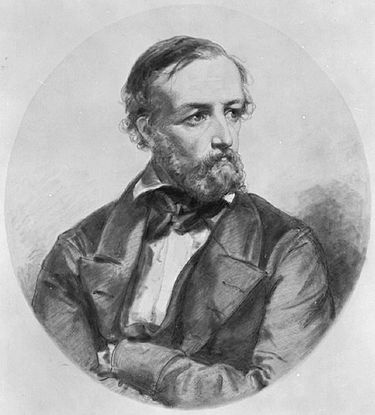
\includegraphics[width=\textwidth]{images/dirichlet.jpg}
                \caption{Johann Dirichlet (src: Wikipedia)}
            \end{figure}
        \end{column}
    \end{columns}

\end{frame}

\begin{frame}
    \frametitle{The Pigeonhole Principle}
    \framesubtitle{Two Definitions}

    \begin{block}{Pigeonhole Principle: Simple Definition}
        If $n$ objects are put in $m$ containers, with $n > m$, then at least one container must contain more than one item.
    \end{block}

    \vspace{10pt}

    \begin{alertblock}{Pigeonhole Principle: Formal Definition}
        Let $S$ be a finite set, with $|S| = n$.
        Let $s_1, \dots, s_k$ be a partition of $S$ in $k$ subsets.
        Then at least one subset $s_i$ of $S$ contains at least $\lceil n/k \rceil$ elements.
    \end{alertblock}
\end{frame}

\begin{frame}
    \frametitle{The Pigeonhole Principle}
    \framesubtitle{A Graphic Interpretation}

    \begin{columns}[t]
        \begin{column}{.45\textwidth}
            \textbf{\textcolor{blue}{Pigeons and Pigeonholes:}}
            \begin{figure}[t]
                \centering
                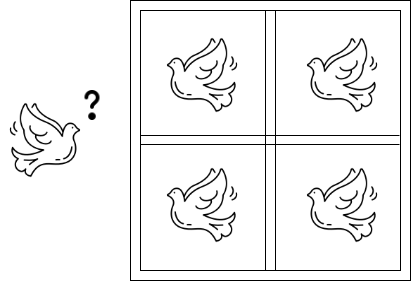
\includegraphics[width=.7\textwidth]{images/pigeons.png}
            \end{figure}
            Two pigeons must share a pigeonhole!
        \end{column}
        \hfill
        \begin{column}{.45\textwidth}
            \textbf{\textcolor{blue}{Cards and Hales:}}
            \begin{figure}[t]
                \centering
                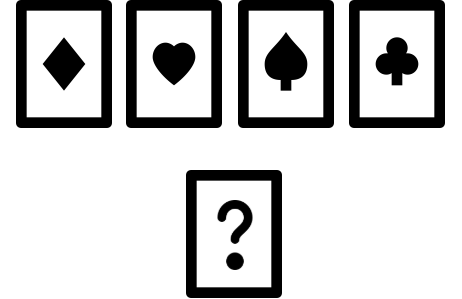
\includegraphics[width=.75\textwidth]{images/cards_hales.png}
            \end{figure}
            We must get two cards of the same suit!
        \end{column}
    \end{columns}

\end{frame}

\begin{frame}
    \frametitle{The Pigeonhole Principle}
    \framesubtitle{Proof by Contradiction}

    \textbf{\textcolor{blue}{Proposition:}}
    \textit{
        Let $S$ be a finite set, with $|S| = n$.
        Let $s_1, \dots, s_k$ be a partition of $S$ in $k$ subsets.
        Then at least one subset $s_i$ of $S$ contains at least $\lceil n/k \rceil$ elements.
    }

    \vspace{5pt}

    \emph{Proof:}
    Let's assume that $k$ divides $n$, and we will \emph{argue by contradiction},

    \begin{enumerate}
        \item Let's assume there is no such $s_i$ with $|s_i| \geq \frac{n}{k}$.
        \item Then it holds, $\forall i \in \lbrace 1, \dots, k \rbrace, |s_i| < \frac{n}{k}$.
        \item But the $s_i$ are a partition of $S$ so their cardinalities must add to $n$. Hence we have:
$$
            n = |S| = \sum_{i = 1}^k |s_i| \overset{2}{<} \sum_{i = 1}^k \frac{n}{k} = n
$$
    \end{enumerate}
    what yields a contradiction ($n < n$) hence our assumption must be false, and hence there exists an $s_i$ with $|s_i| \geq \frac{n}{k}$. \hfill $\qed$

    \vspace{10pt}

    \begin{center}
        \textbf{\textcolor{blue}{Exercise:}} What if $k$ does not divide $n$?
    \end{center}
\end{frame}

\begin{frame}
    \frametitle{Interesting Applications}
    \framesubtitle{Hairs in London}

    \vspace{-20pt}

    Using this principle, we can prove that at least \textbf{two people} in London have the \textbf{\textcolor{blue}{same number of hairs}} in their head:

    \begin{enumerate}
        \item<2-> A human (non-bald) has, on average, $150$ thousand hairs in their head.
        \item<3-> We \emph{can assume} no one has more than $1$ million hairs in their head.
        \item<4-> Let $S$ be the number of persons in London, and $s_1, \dots, s_{10^6}$ our partition.
            Clearly $|S| > 10^6$.
        \item<5-> A person $p$ belongs to $s_i$ iff $p$ has $i$ hairs.
    \end{enumerate}

    \only<6->{
        Apply the principle and \textbf{\textcolor{blue}{at least two people}} in $S$ fall in the same partition and hence have the same number of hairs.
    }

    \only<7->{
        \begin{alertblock}{Observation}
            Note that the principle ensures the existence of a container with at least two elements, it does not argue about the exact number, neither on overlaps.
            For that, probability distributions need to be used.
        \end{alertblock}
    }
\end{frame}

\begin{frame}
    \frametitle{Interesting Applications}
    \framesubtitle{Erd\H{o}s-Szekeres Theorem}

    % Mention that they have seen sequences in 145
    \begin{alertblock}{Theorem (Erd\H{o}s-Szekeres, 1936)}
        Let $r,s$ be two natural numbers.
        Any sequence of distinct real numbers with length at least $(r-1)(s-1) + 1$ contains a monotonically increasing subsequence of length $r$ or a monotonically decreasing subsequence of length $s$.
    \end{alertblock}

    \vspace{10pt}

    \only<2->{
        \begin{itemize}
            \item Proven in 1936 by Paul Erd\H{o}s and George Szekeres
            \item It has applications in several domains: graph theory, combinatorics, geometry, ...
            \item What if the sequence is infinite? Check \textcolor{blue}{Ramsey's} theorem.
        \end{itemize}
    }

\end{frame}

\begin{frame}
    \frametitle{Interesting Applications}
    \framesubtitle{Erd\H{o}s-Szekeres Theorem - Proof}

    \vspace{-10pt}

    \emph{Proof:}
    Let $a_1, \dots, a_{(r-1)(s-1) + 1}$ be our sequence of \emph{distinct} real numbers.\\
    For each $a_i$, let us label it with a pair $(u_i, d_i)$ where:
    \begin{itemize}
        \item $u_i$ is the length of the longest increasing subsequence ending in $a_i$,
        \item $d_i$ is the length of the longest decreasing subsequence ending in $a_i$,
    \end{itemize}
    \emph{\textcolor{blue}{Observation:}} given the previous definition, observe that, if $i < j$,
    \begin{itemize}
        \item[(i)] $a_i < a_j \Longrightarrow u_i < u_j$
        \item[(ii)] $a_i > a_j \Longrightarrow d_i < d_j$
    \end{itemize}
    Argument by contradiction: let's assume there is \textbf{no} increasing subsequence of length $r$ \textbf{and no} decreasing subsequence of length $s$.
    Then $u_i \leq r-1$ and $d_i \leq s-1$ hence we have a total of $(r-1)(s-1)$ possible labellings. By the pigeonhole principle,
    $$ \exists a_i, a_j \text{ s.t. } u_i = u_j \wedge d_i = d_j \Rightarrow a_i = a_j \hspace{5pt} \text{, but the $a_i$ were all distinct!}$$
    \hspace{20pt}Hence our assumption was false and there exists \textbf{either} an increasing subsequence of\\
    \hspace{40pt}length $r$ \textbf{or} a decreasing one of length $s$. \hfill $\qed$
\end{frame}

\begin{frame}
    \frametitle{Questions \& Debate}

    \begin{center}

        \Large
        \textbf{\textcolor{blue}{Questions are now welcome!}}

        \href{mailto:carlossegarragonzalez@gmail.com}{carlossegarragonzalez@gmail.com}

    \end{center}


\end{frame}

\end{document}
